\documentclass[12pt]{article}
\newcommand\tab[1][0.5cm]{\hspace*{#1}}
\usepackage[utf8]{inputenc}
\usepackage{listings}
\usepackage{hyperref}
\usepackage{color}
\pagenumbering{gobble}
\usepackage{changepage}
\usepackage{titletoc}
\usepackage{titlesec}
\usepackage{multicol}
\usepackage{graphicx}

\usepackage{makecell}

\definecolor{codegreen}{rgb}{0,0.6,0}
\definecolor{codegray}{rgb}{0.5,0.5,0.5}
\definecolor{codepurple}{rgb}{0.58,0,0.82}
\definecolor{backcolour}{rgb}{0.95,0.95,0.92}

\hypersetup{
	colorlinks,
	citecolor=black,
	filecolor=black,
	linkcolor=black,
	urlcolor=black
}

\lstdefinestyle{mystyle}{
	backgroundcolor=\color{backcolour},   
	commentstyle=\color{codegreen},
	keywordstyle=\color{magenta},
	numberstyle=\tiny\color{codegray},
	stringstyle=\color{codepurple},
	basicstyle=\footnotesize\ttfamily,
	breakatwhitespace=false,         
	breaklines=true,                 
	captionpos=b,                    
	keepspaces=true,                 
	numbers=left,                    
	numbersep=5pt,                  
	showspaces=false,                
	showstringspaces=false,
	showtabs=false,                  
	tabsize=2
}

\lstset{style=mystyle}

\newcommand{\titledate}[2][2.5in]{%
	\noindent%
	\begin{tabular}{@{}p{#1}@{}}
		\\ \hline \\[-.75\normalbaselineskip]
		#2
	\end{tabular} \hspace{1in}
	\begin{tabular}{@{}p{#1}@{}}
		\\ \hline \\[-.75\normalbaselineskip]
		Date
	\end{tabular}
}

\titleformat{\section}{\normalfont\Large\bfseries}{}{0pt}{}

% for forcing tables to fit
\usepackage{changepage}

\begin{document}
	

\begin{titlepage}
	
\author{Eric Pereira}
\date{October 24\textsuperscript{th}, 2019}
\title{CSE4501 -- Vulnerability Research:\\Midterm}

\maketitle

\end{titlepage}

\titlecontents{section}[0em]
{\vskip 0.5ex}%
{\scshape}% numbered sections formattin
{\itshape}% unnumbered sections formatting
{}%

\tableofcontents

\newpage \pagenumbering{arabic}

\section{Introduction}:

Snoogins OS is a brand new, state of the art, high tech, machine blockhain learning operating system that has incredibly useful
commands. It, however, seems to possibly have at least 3 vulnerabilities. For finding at least 3 vulnerabilities I will be paid 
with 100 points (that's more points than I've ever seen in my life!). With that said, let's start looking for the the first 
vulnerability, referenced in the \texttt{WinFlag1} function. 

%%%%%%%%%%%%%%%%%%%%%%%%%%%%%%%%%%%%%%%%%%%%%%%%%%%%%%%%%%%%%%%%%%%%%%%%%%%%%%%%%%
%                                                                                %
%                                   WINFLAG1                                     %
%                                                                                %
%%%%%%%%%%%%%%%%%%%%%%%%%%%%%%%%%%%%%%%%%%%%%%%%%%%%%%%%%%%%%%%%%%%%%%%%%%%%%%%%%%

\section{WinFlag1}

\tab Upon Reviewing, My first instinct was to look immediately for the \texttt{WinFlag} functions and cross reference
them to see where they are called. The first flag, \texttt{WinFlag1} can be found in another function, the \texttt{cmdexit}
function. This function is called when you run the Snoogins OS and type the command \texttt{exit}. I then went to observe the 
specific code to see exactly what was happening. The graphical view of the code looks like:
\begin{center}
	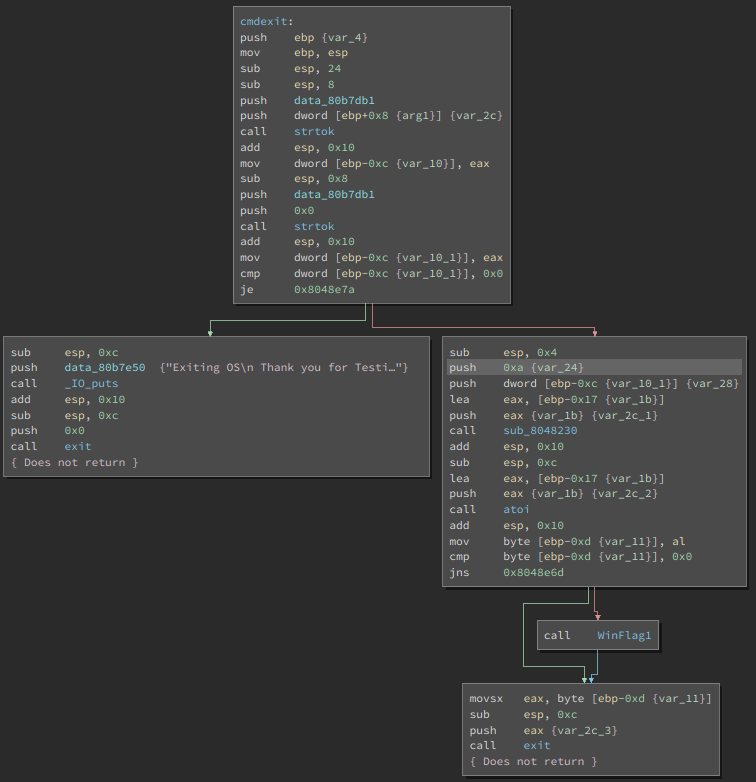
\includegraphics[scale=.46]{photos/winflagone.png}
\end{center}

What I see is right above where Winflag would be called, a variable is created with allocated memory size of 10 bytes, that would
be seem near the \texttt{strtok} function. This seems to be some sort of arguement that is called in conjunction with exit, 
and scanned in when exit is called. If exit has a non-null arguement of some sort it goes to the path on the right, and then
it seems that there is a check of some sort on the stack after 10 bytes. So, in order to get the first flag you have to give some
input of at least 11 characters passed in with the \texttt{exit} command. Let's see what happens when we run this command. 
\begin{center}
	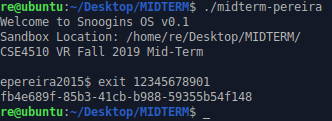
\includegraphics[scale=1]{photos/winflag1.png}
\end{center}

There it is! The first vulnerability, represented by the UUID or GUID (or whatever term you want to call them) which is: 
\begin{center}
	\texttt{fb4e689f-85b3-41cb-b988-59355b54f148}.
\end{center}



%%%%%%%%%%%%%%%%%%%%%%%%%%%%%%%%%%%%%%%%%%%%%%%%%%%%%%%%%%%%%%%%%%%%%%%%%%%%%%%%%%
%                                                                                %
%                                   WINFLAG2                                     %
%                                                                                %
%%%%%%%%%%%%%%%%%%%%%%%%%%%%%%%%%%%%%%%%%%%%%%%%%%%%%%%%%%%%%%%%%%%%%%%%%%%%%%%%%%

\section{WinFlag2}

\tab I initially had quite a bit of trouble with the second flag, I went to use the tool Ghidra for more help as a result. 
I had a strange amount of difficulty cross referencing the \texttt{WinFlag2} function. Very strange. I then opened up in IDA64 only
to get a notification that ``There are no xrefs to WinFlga2". That, is interesting, so I supposed I am chasing the wrong flag, or I
need to find some way to run the flag indirectly. I am suspecting that we need to generate the buffer of data plus the address of the
function in order to run it. Let's see if we can attempt to do this. In order to do this, however, we have to look and find a potential exploit
where we can place the value of a specific address into a function. 

\end{document}
